%%
%% Copyright (C) Hochschule Esslingen, 2011
%%
%% $Id: example.tex 131 2011-10-16 01:11:22Z uwe $
%%
%% This work may be distributed and/or modified under the
%% conditions of the LaTeX Project Public License, either version 1.3
%% of this license or (at your option) any later version.
%% The latest version of this license is in
%%   http://www.latex-project.org/lppl.txt
%% and version 1.3 or later is part of all distributions of LaTeX
%% version 2005/12/01 or later.

%\makeglossaries

\begin{document}

% If you wish to uncover everything in a step-wise fashion, uncomment
% the following command: 
% \beamerdefaultoverlayspecification{<+->}

\mode<article>{\maketitle}

\begin{frame}
  \titlepage
\end{frame}

\ifoverview
% ----- No TOC in course overview
\else
\begin{frame}{Content}
  \tableofcontents
\end{frame}
\fi

\ifoverview
\section{Introduction: Chapter 1: Distributed Real-Time Systems}


Lecturer: Vikas Agrawal, vikas.agrawal@hs-esslingen.de,
Room F 01.301

\section{Literature for this lecture}\label{literature-for-this-lecture}

\begin{longtable}[c]{@{}l@{}}
\toprule
\textbf{Text books for this lecture}\tabularnewline
{[}1.1{]}Kopetz, H.: Distributed Real-Time Systems, Springer 2008\tabularnewline
{[}1.2{]}Buttazzo, G.: Hard Real-Time Computing Systems, Springer 2005\tabularnewline
\bottomrule
\end{longtable}

\begin{longtable}[c]{@{}l@{}}
\toprule
\textbf{Complementing texts}

\emph{Some books complementing the material treated in this lecture}\tabularnewline
{[}2.1{]}Liu, J.S.: Real-Time Systems, Prentice Hall 2000\tabularnewline
{[}2.2{]}Vérissimo, P; Rodrigues, L.: Distributed Systems for System Architects, Kluwer 2001\tabularnewline
{[}2.3{]}Laplante, P.: Real-Time Systems Design and Analysis, IEEE Press, 2004\tabularnewline
{[}2.4{]}Halbwachs, N.: Synchronous Programming of Reactive Systems, Kluwer 1993\tabularnewline
{[}2.5{]}Zimmermann, W.; Schmidgall, R.: Bussysteme in der Fahrzeugtechnik, Vieweg 2006 (German only)\tabularnewline
\bottomrule
\end{longtable}

\begin{longtable}[c]{@{}l@{}}
\toprule
\textbf{Journal Articles and Web Documents}

\emph{Original journal articles and documents from the web pertaining to this lecture}\tabularnewline
{[}3.0{]}Albert, A.:Comparison of Event-Triggered and Time-Triggered Concepts with Regard to Distributed Control Systems, Embedded World, 2004, Nürnberg\tabularnewline
%http://www.semiconductors.bosch.de/pdf/embedded_world_04_albert.pdf
{[}3.1{]}Müller, B.; Führer, T.; Hartwich, F.; Hugel, R.; Weiler, H.: Fault Tolerant TTCAN Networks, Proceedings 8th International CAN Conference; 2002; Las Vegas, NV\tabularnewline
%http://www.semiconductors.bosch.de/pdf/Fault_Tolerant_TTCAN.pdf\tabularnewline
\bottomrule
\end{longtable}

\begin{frame}{Introduction}{Part 1}
    \begin{block}{Overview}
Chapter 1	  The Real-Time Environment\\
Chapter 2	  Distributed Real-Time Systems\\
Chapter 3	  Global Time\\
Chapter 4	  Modeling Real-Time Systems\\
Chapter 5	  Real-Time Entities and Images\\
Chapter 6	  Fault Tolerance\\
Chapter 7	  Real-Time Communication\\
Chapter 8	  Time-Triggered Protocols\\
Chapter 9	  Input and Output\\
Chapter 10	Real-Time Operating Systems: OSEK and AUTOSAR\\
Chapter 11	Real-Time Scheduling\\
Chapter 12	Validation
\end{block}
\end{frame}


\begin{frame}{Introduction}{Part 1}
    \begin{block}{The Real-Time Environment}
\begin{itemize}
\item
  Definition of a real-time system.
\item
  Simple model with operator, computer system, and controlled object.
\item
  Introduction of distributed real-time systems.
\item
  Hard real-time systems and soft real-time systems.
\item
  Functional, temporal, and dependability requirements.
\item
  Sphere of control
\item
  Event-triggered versus time-triggered systems.
\end{itemize}
\end{block}
\end{frame}

\begin{frame}{Introduction}{Part 2}
    \begin{block}{Distributed Real-Time Systems}
\begin{itemize}
\item
  Distributed system architecture overview, clusters, nodes,
  communication network
\item
  Structure of node with host computer, communication network interface,
  communication controller
\item
  Event and state messages, gateways.
\item
  Concept of composability.
\item
  Event- and time-triggered communication systems.
\item
  Scalability, dependability, issues of physical installation.
\end{itemize}
\end{block}
\end{frame}


\begin{frame}{Introduction}{Part 3}
    \begin{block}{Global Time}
\begin{itemize}
\item
  Notions of causal order, temporal order, and delivery order
\item
  External observers, reference clocks, and global time base
\item
  Sparse time base to view event order in a distributed real-time system
\item
  Internal clock synchronization to compensate for drift offset.
  Influence of the communication system jitter on the precision of the
  global time base.
\item
  External time synchronization, time gateways, and the Internet network
  time protocol (NTP)
\end{itemize}
\end{block}
\end{frame}


\begin{frame}{Introduction}{Part 4}
    \begin{block}{Modeling Real-Time Systems}
\begin{itemize}
\item
  Introduction of a conceptual model for real-time systems
\item
  Tasks, nodes, fault-tolerant units, clusters
\item
  Simple and complex tasks
\item
  Interface placement and interface layout
\item
  Temporal control and logical control
\item
  The history state
\end{itemize}
\end{block}
\end{frame}


\begin{frame}{Introduction}{Part 5}
    \begin{block}{Real-Time Entities and Images}
\begin{itemize}
\item
  Real-time entities
\item
  Observations, state and event observations
\item
  Real-time images as current picture of real-time entity, and real-time
  objects
\item
  Temporal accuracy and state estimation to improve real-time image
  accuracy
\item
  Permanence in case of race conditions and idempotency with replicated
  messages
\item
  Replica determinism to implement fault-tolerance by active redundancy
\end{itemize}
\end{block}
\end{frame}


\begin{frame}{Introduction}{Part 6}
    \begin{block}{Fault Tolerance}
\begin{itemize}
\item
  Failures, Errors, and Faults
\item
  Error Detection
\item
  A Node as a Unit of Failure
\item
  Fault Tolerant Units
\item
  Reintegration of a Repaired Node
\item
  Design Diversity
\end{itemize}
\end{block}
\end{frame}


\begin{frame}{Introduction}{Part 7}
    \begin{block}{Real-Time Communication}
\begin{itemize}
\item
  Real-Time Communication Requirements
\item
  Flow Control
\item
  OSI Protocols for Real-Time
\item
  Fundamental Conflicts in Protocol Design
\item
  Media-Access Protocols
\item
  Performance Comparison: ET versus TT
\item
  The Physical Layer
\end{itemize}
\end{block}
\end{frame}


\begin{frame}{Introduction}{Part 8}
    \begin{block}{Time-Triggered Protocols}
\begin{itemize}
\item
  Introduction to Time-Triggered Protocols
\item
  Overview of the TTP/C Protocol Layers
\item
  The Basic CNI
\item
  Internal Operation of TTP/C
\item
  TTP/A for Field Bus Applications
\end{itemize}
\end{block}
\end{frame}


\begin{frame}{Introduction}{Part 9}
    \begin{block}{Input and Output}
\begin{itemize}
\item
  The dual role of time
\item
  Agreement protocol
\item
  Sampling and polling
\item
  Interrupts
\item
  Sensors and actuators
\item
  Physical installation
\end{itemize}
\end{block}
\end{frame}


\begin{frame}{Introduction}{Part 10}
    \begin{block}{Real-Time Operating Systems: OSEK and AUTOSAR}
\begin{itemize}
\item
  Task management
\item
  Interprocess communication
\item
  Time management
\item
  Error detection
\item
  OSEK and AUTOSAR
\end{itemize}
\end{block}
\end{frame}


\begin{frame}{Introduction}{Part 11}
    \begin{block}{Real-Time Scheduling}
\begin{itemize}
\item
  The scheduling problem
\item
  The adversary problem
\item
  Dynamic scheduling, dynamic priority servers
\item
  Static scheduling, fixed priority servers
\end{itemize}
\end{block}
\end{frame}


\begin{frame}{Introduction}{Part 12}
    \begin{block}{Validation}
\begin{itemize}
\item
  Building a Convincing Safety Case
\item
  Formal Methods
\item
  Testing
\item
  Fault Injection
\item
  Dependability Analysis
\end{itemize}
\end{block}
\end{frame}

\fi

\ifpartI
\begin{enumerate}
\item ~
  \section{Chapter 1}\label{chapter-1}

  \begin{enumerate}
  \item ~
    \subsection{The Real-Time
    Environment}\label{the-real-time-environment}
  \end{enumerate}
\end{enumerate}

Overview 2

\begin{enumerate}
\def\labelenumi{\arabic{enumi}.}
\item
  When is a Computer System Real-Time? 3
\item
  Functional Requirements 6
\item
  Temporal Requirements 13
\item
  Dependability Requirements 17
\item
  Classification of Real-Time Systems 21
\item
  Automotive Real-Time Systems 23
\end{enumerate}

1.7 Points to Remember 25

\subsection{Overview}\label{overview}

\begin{itemize}
\item
  Describing the environment of real-time computer systems from various
  perspectives
\item
  Definition of a real-time system with discussion of functional and
  metafunctional requirements
\item
  Emphasis on temporal requirements derived from control applications;
  satisfying performance criteria in control applications; quality of
  control
\item
  Difference between hard and soft real-time systems
\item
  Soft real-time systems may follow a less rigorous design approach,
  accepting failure under peak load conditions due to economic arguments
\item
  In hard real-time systems failure is unacceptable; safety of a design
  under all circumstances must often be demonstrated to a certification
  agency
\item
  Automobiles as assembly of many dedicated real-time systems
\end{itemize}

\textbf{1.1} \protect\hypertarget{teil2}{}{}\textbf{When is a Computer
System Real-Time?}

\emph{A real-time computer system is a computer system in which the
correctness of the system behavior depends not only on the logical
results of the computations, but also on the physical instant at which
these results are produced.}

A real-time computer system is always part of a larger system, the
real-time system.

We decompose a real-time system into a set of subsystems called
clusters.

\begin{longtable}[c]{@{}ll@{}}
\toprule
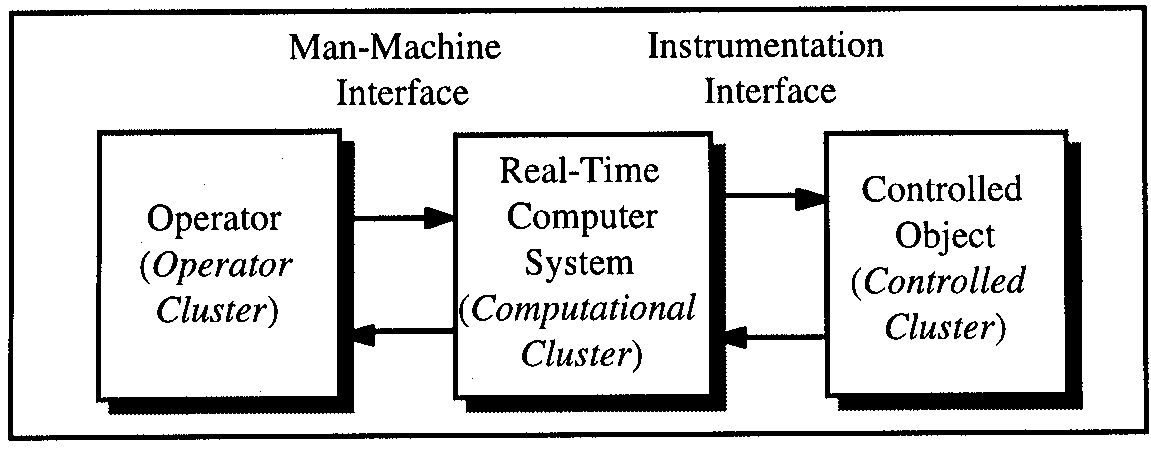
\includegraphics[width=7.51736in,height=2.93681in]{media/Fig_1_1.png} &
Man-Machine-Interface: keyboard, mouse, screen

Instrumentation-Interface: sensors and actuators, transforming physical
signals into a digital form and vice versa\tabularnewline
\bottomrule
\end{longtable}

The controlled object and the operator form the environment of the
real-time computer system. Not every node has both, a man-machine
interface and an instrumentation interface.

A distributed real-time computer system consists of a set of computer
nodes interconnected by a real-time communication network.

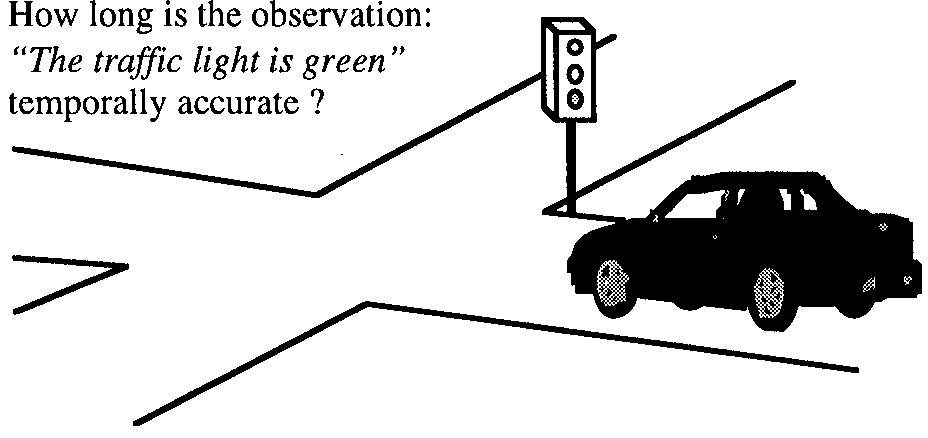
\includegraphics[width=7.02222in,height=3.35556in]{media/Fig_1_2.png}

A real-time computer system must react to stimuli from the controlled
object or operator within time intervals dictated by the environment.

The instant at which the result must have been produced is called a
deadline.

Soft deadline: result has some utility passed this instant in time.

Firm deadline: result has no or very little utility past this instant in
time.

Hard deadline: catastrophic failure when result is produced past this
instant in time.

Hard real-time computer system or safety-critical real-time computer
system:

\begin{itemize}
\item
  A real-time system that must meet at least one hard deadline.
\end{itemize}

Soft real-time computer system:

\begin{itemize}
\item
  A real-time computer system for which no hard deadline exists.
\end{itemize}

\textbf{1.2} \protect\hypertarget{teil3}{}{}\textbf{Functional
Requirements}

Functional Requirements are grouped into

\begin{itemize}
\item
  Data collection requirements
\item
  Direct digital control requirements
\item
  Man-machine interaction requirements

  \begin{enumerate}
  \item ~
    \subsection{Data Collection}\label{data-collection}
  \end{enumerate}
\end{itemize}

A controlled object (car, industrial plant) changes its state as a
function of time.

Current state: values of all state variables at this moment

Example: speed of car, position of switches on dashboard, position of
piston in a cylinder

We are normally only interested in a subset of state variables
significant for our purpose:

\begin{itemize}
\item
  A significant state variable is called a real-time (RT) entity.
\end{itemize}

Every RT entity is in the sphere of control (SOC) of a subsystem, i.e.,
it belongs to a subsystem that can change the value of that RT entity.

Outside that SOC the value of that entity can only be observed, not
modified.

Thus, we have the following functional requirements:

\begin{itemize}
\item
  Observation of the RT entities in a controlled object
\item
  Collection of these observations
\end{itemize}

An observation of an RT entity is represented by a real-time (RT) image.

Example for accuracy interval:

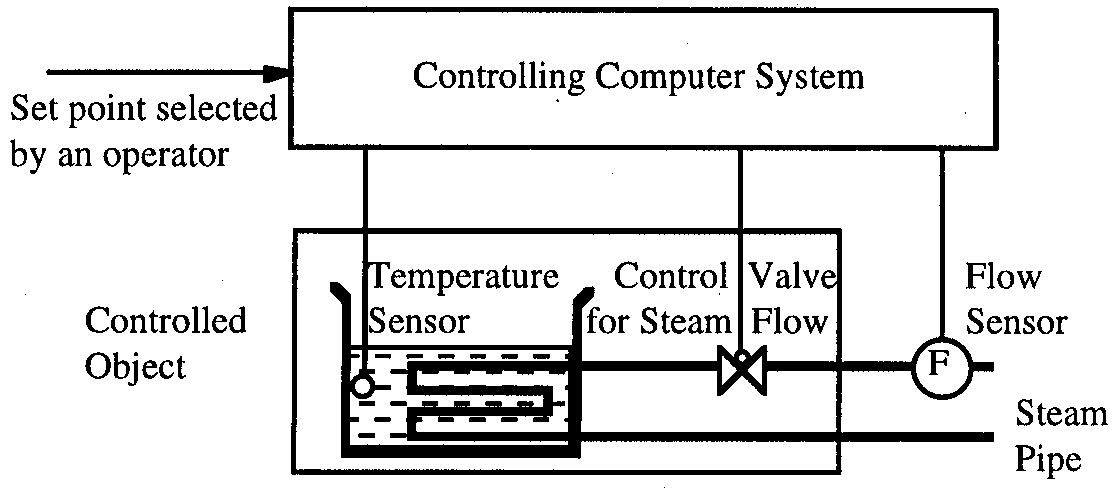
\includegraphics[width=6.67708in,height=3.05208in]{media/Fig_1_3.png}

If the information „traffic light is green`` is used outside its
accuracy interval, a collision may occur.

The set of all temporally accurate RT images of the controlled object is
called the real-time database.

The RT database must be updated whenever an RT entity changes its value.

The update can be performed periodically with a fixed period
(time-triggered (TT) observation).

The update can be performed immediately after a state change in the RT
entity, which constitutes an event (event-triggered (ET) observation).

\textbf{Signal conditioning}

Signal conditioning encompasses all processing steps to obtain
meaningful measured data from physical sensor data (raw data element,
e.g. a voltage). Typical processing steps:

\begin{itemize}
\item
  filtering and averaging
\item
  plausibility checks
\item
  calibration and transformation
\end{itemize}

Agreed data element: a data element judged to be a correct RT image of
the corresponding RT entity.

\textbf{Alarm monitoring}

Alarm monitoring serves to detect abnormal behaviour by continuous
observation of RT entities.

Example: rupture of a pipe in a chemical plant will cause many RT
entities (pressures, temperatures, liquid levels) deviate from their
normal operating ranges.

The rupture will lead to a set of correlated alarms, which is called an
alarm shower.

The computer system must detect and display these alarms, and must try
to identify the primary event (the initial cause of the alarm).

Alarms are logged with the exact time at which they occur. The time
stamp helps to eliminate secondary alarms.

A situation that occurs infrequently but is of great concern when it
does is called a rare-event situation. Rare-event performance validation
is a great challenge (e.g. nuclear plants).

\subsection{Direct Digital Control}\label{direct-digital-control}

Many real-time computer systems must calculate set points for the
actuators and control the controlled object directly. Example: engine
controller

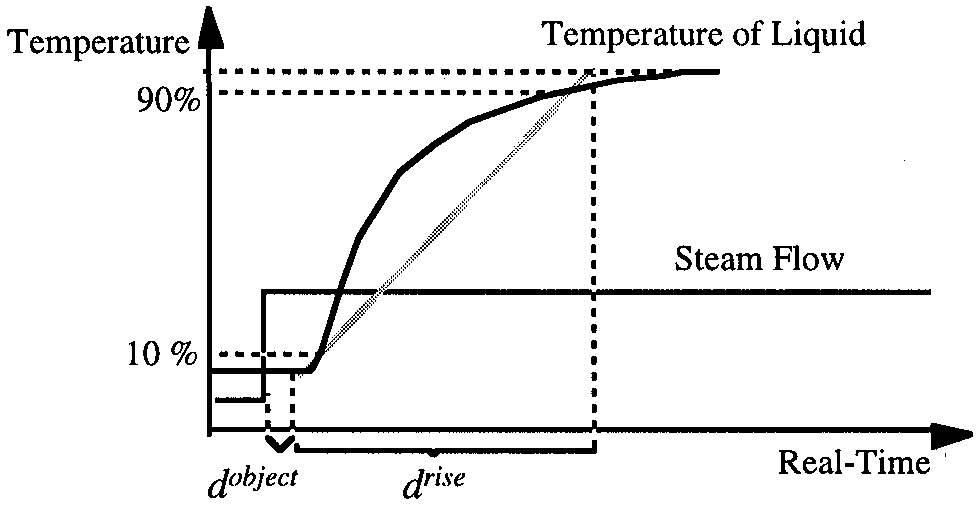
\includegraphics[width=6.85069in,height=5.00278in]{media/Fig_1_4.png}

Control applications are highly regular, consisting of an infinite
sequence of control periods:

\begin{itemize}
\item
  Sampling of the RT entity
\item
  Execution of the control algorithm to calculate a new set point
\item
  Output of set point to actuator
\end{itemize}

Design of control algorithms is topic of field of control engineering.

\subsection{Man-Machine Interaction}\label{man-machine-interaction}

A real-time computer system must inform the operator of the current
state of the controlled object, and must assist the operator in
controlling the machine or plant object.

The man-machine interface in safety-critical real-time systems is of
utmost importance. A bad design can result in catastrophic failures.

\begin{longtable}[c]{@{}ll@{}}
\toprule
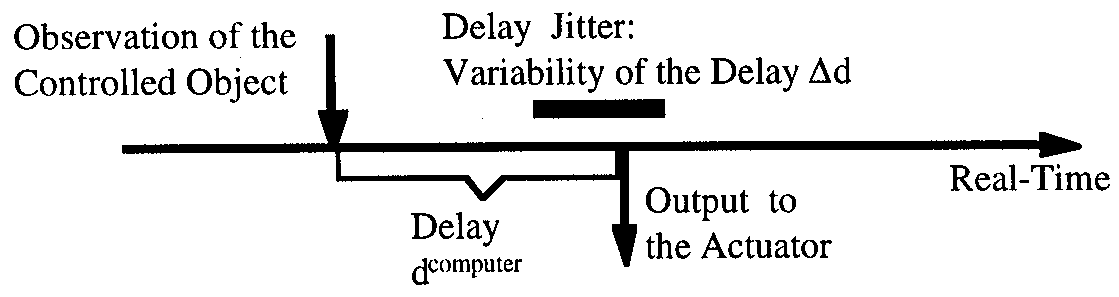
\includegraphics[width=5.14375in,height=3.70694in]{media/Fig_1_5.png} &
Automotive examples:

\begin{itemize}
\item
  Dashboard
\item
  Joystick
\item
  Steering wheel
\item
  Brake, accelerator pedal
\end{itemize}

This topic justifies a lecture on its own, and is not dealt with any
further here.\tabularnewline
\bottomrule
\end{longtable}

\textbf{1.3} \protect\hypertarget{teil4}{}{}\textbf{Temporal
Requirements}

\begin{itemize}
\item
  Most stringent temporal demands come from control loops, e.g. control
  of fast mechanical processes such as automotive engines
\item
  Requirements at the MMI are less stringent (human perception delay is
  between 50-100 ms)
\item
  Example for a simple control loop: control steam flow through pipe
  such that liquid temperature remains at set point.
\end{itemize}

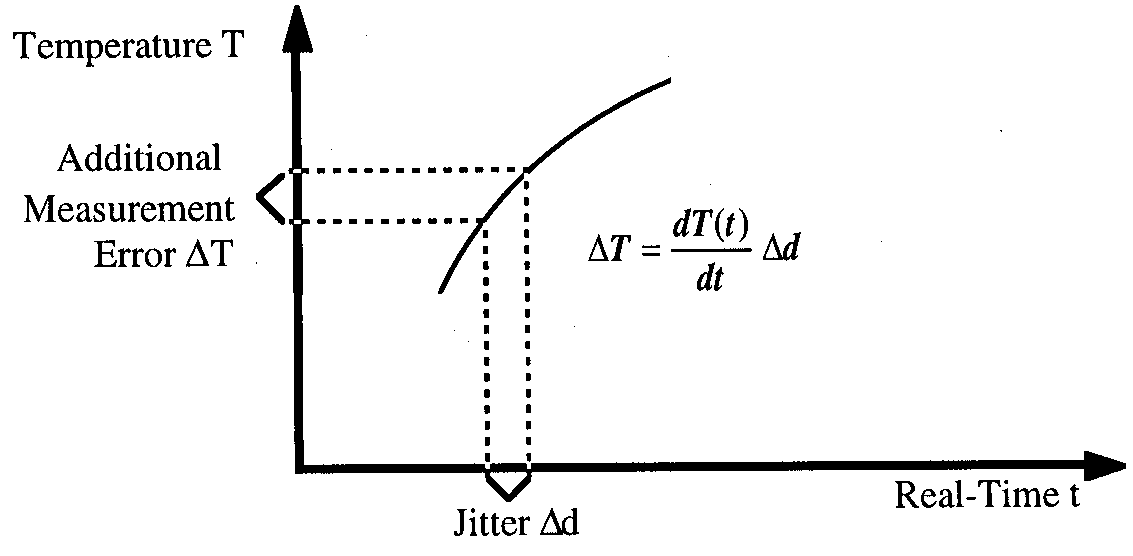
\includegraphics[width=7.39792in,height=3.25903in]{media/Fig_1_6.png}

Behavior of liquid temperate when steam flow is increased instantly by a
fixed amount: response function of the temperature.

Response function characterized by two temporal parameters: object delay
\emph{d\textsuperscript{object}} or process lag and rise time
\emph{d\textsuperscript{rise}} of the temperature

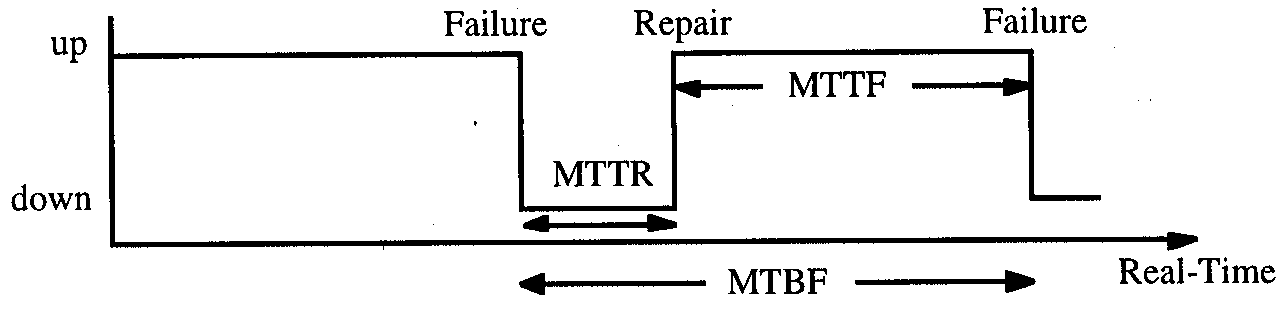
\includegraphics[width=7.02153in,height=3.66736in]{media/Fig_1_7.png}

Controlling computer system samples temperature of vessel periodically
with sampling period \emph{d\textsuperscript{sample}}. The sampling
frequency is \emph{f\textsuperscript{sample}} = \emph{1/
d\textsuperscript{sample}} .

Rule of thumb: sampling period should be less than one-tenth of the rise
time \emph{d\textsuperscript{rise}} of controlled object to obtain
quasi-continuous behavior (\emph{d\textsuperscript{sample} \textless{}
d\textsuperscript{rise}}/\emph{10}).

The computer system calculates the new value for the control variable,
and outputs it to the control valve after some delay, called the
computer delay \emph{d\textsuperscript{computer}}. The computer delay
should be less than the sampling period
\emph{d\textsuperscript{sample}}.

The jitter \emph{Δd\textsuperscript{computer}} is the difference between
the maximum and minimum computer delay. It should be small compared to
the computer delay \emph{d\textsuperscript{computer}} (µs to ms). The
jitter can be interpreted as causing an additional error of the
temperature \emph{ΔT.}

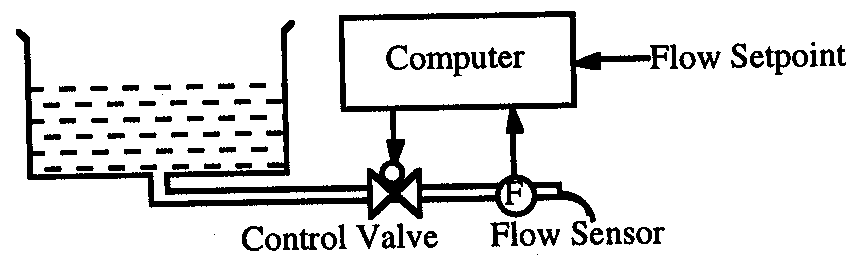
\includegraphics[width=6.64444in,height=3.26042in]{media/Fig_1_8.png}

The dead time \emph{d\textsuperscript{deadtme }}is the time interval
between the observation of the RT entity and the start of a reaction of
the controlled object due to a computer action.

The dead time is \emph{d\textsuperscript{object}} +
\emph{d\textsuperscript{computer}}.

Dead time reduces stability of the control loop, and should thus be as
small as possible.

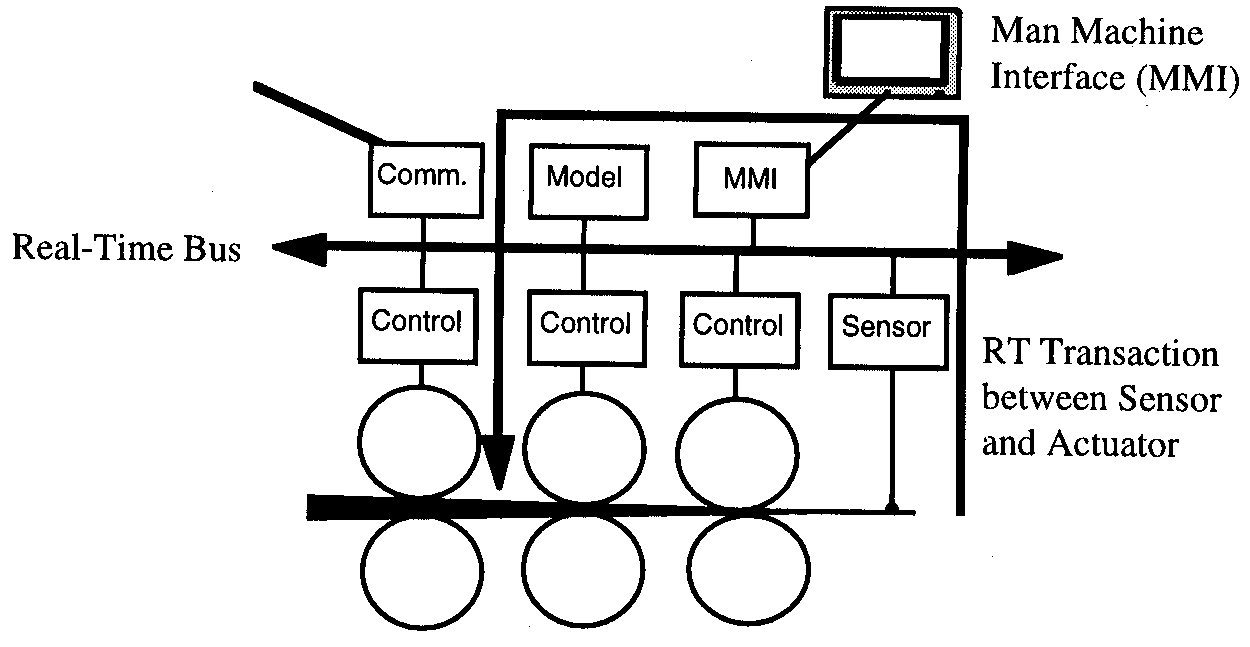
\includegraphics[width=7.50625in,height=1.99236in]{media/Fig_1_9.png}

Hard real-time applications are, by definition, safety-critical. Errors
must therefore be detected within a short time with high probability.
The required error detection latency must be in the order of magnitude
of the sampling period of the fastest control loop.

\textbf{1.4} \protect\hypertarget{teil5}{}{}\textbf{Dependability
Requirements}

Dependability is determined by:

\begin{itemize}
\item
  Reliability
\item
  Safety
\item
  Maintainability
\item
  Availability
\item
  Security
\end{itemize}

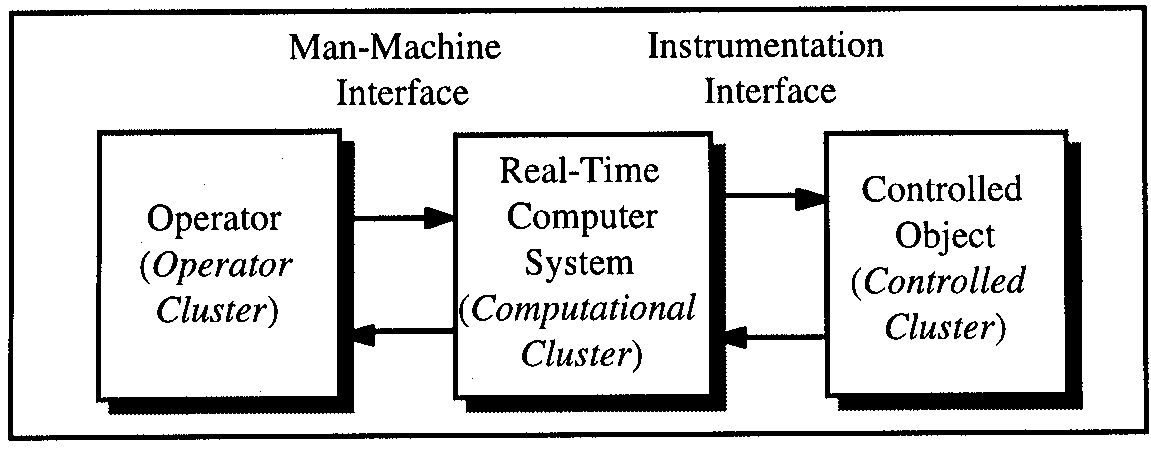
\includegraphics[width=7.77292in,height=1.88542in]{media/Fig_1_1.png}

\textbf{Reliability}

Reliability R(t) is the probability that a system will provide the
specified service until time \emph{t}, given that the system was
operational at time \emph{t\textsubscript{0}}.

If a system has a constant failure rate \emph{λ} \emph{failures/hour},
then \emph{R(t)} is given by

\emph{R(t) = exp(-λ (t-t0))} (with t and t\textsubscript{0} given in
hours)

The inverse of the failure rate \emph{1/λ = MTTF} is called the
Mean-Time-To-Failure (in hours).

\textbf{Safety}

Safety is reliability regarding critical failure modes (malign failure
modes). Examples of malign failures:

\begin{itemize}
\item
  airplane crash due to a failure in the flight-control system
\item
  automobile accident due to a failure in the computer controlled
  braking system
\end{itemize}

Hard real-time systems must have a failure rate conforming to ultrahigh
reliability requirements (\emph{Lambda 10\textsuperscript{-9}
failures/hour} or less). Example: one such failure per one million cars
per year, when car is operated one hour per day.

\textbf{Maintainability}

Maintainability is a measure of the time required to repair a system
after the occurrence of a benign failure (non safety-critical failure).
It is measured by the probability M(d) that the system is restored
within a time interval \emph{d} after the failure.

Similar to reliability, there is a repair rate \emph{µ} ; the inverse of
the repair rate \emph{1/µ = MTTR} is called the Mean-Time-To-Repair (in
hours).

Reliability and maintainability are in conflict to each other (e.g.
soldered connection vs. plug). Many replaceable units improve
maintainability and reduce reliability. In automotive market typically
OEMs decide for reliability at the cost of maintainability.

\textbf{Availability}

Availability is a measure of the delivery of correct service with
respect to the alternation of correct and incorrect service. It is
measured by the fraction of time the system is ready to provide the
service.

In systems with constant failure and repair rates, the reliability
(\emph{MTTF}), maintainability (\emph{MMTR}) and availability (\emph{A})
measures are related by

\emph{A = MTTF / (MTTF+MTTR)}

The sum of \emph{MTTF} and \emph{MTTR} is called the Mean Time Between
Failures (\emph{MTBF}).

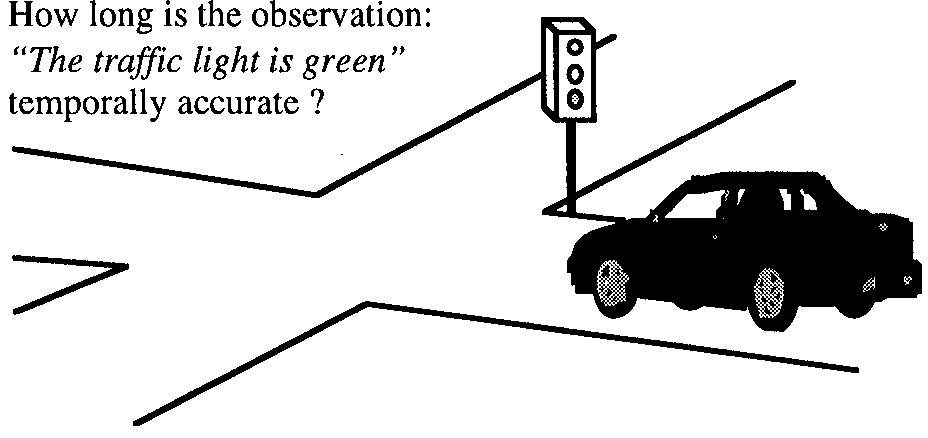
\includegraphics[width=7.63958in,height=1.85347in]{media/Fig_1_2.png}

A high availability can be achieved by high \emph{MTTF} or by a short
\emph{MTTR}.

\textbf{Security}

Security is the ability of a system to prevent unauthorized access to
information or services. Examples in the automotive context are:

\begin{itemize}
\item
  Ignition lock for theft avoidance
\item
  Car access with lock system
\item
  Protection against software reverse engineering and manipulation
\end{itemize}

There is no standardized quantitative measure for security.

\textbf{1.5} \protect\hypertarget{teil6}{}{}\textbf{Classification of
Real-Time Systems}

\textbf{Fail-Safe versus Fail-Operational}

Fail safe: controlled object can enter a safe state where nothing bad
can happen (e.g. all traffic lights switched to red, all trains
stopped). Fail-safeness is property of controlled object, not of
computer system.

Fail-operational: system must be still operational in case of failure
(airplane, no safe state).

\textbf{Guaranteed-Response versus Best-Effort}

We assume some peak load and a fault model. If we can buy design
guarantee adequate responses under all conditions, without reverting to
probability arguments, we can speak of a system with a guaranteed
response. Guaranteed response systems usually require careful planning
and extensive analysis during the design phase.

In case we cannot guarantee adequate response by design, we speak of a
best effort system.

It is very difficult to demonstrate that a best-effort design operates
correctly under rare event scenarios. There is always a fall back
default value in case the requested value cannot be responded in real
time.

\textbf{Resource-Adequate versus Resource-Inadequate}

Guaranteed response systems must have enough resources to handle a
specified peak load and fault scenario. Due to economic reasons many non
safety-critical real-time systems are based on the principle of resource
inadequacy.

\textbf{Event-Triggered versus Time-Triggered}

In the event-triggered approach, all communication and processing
activities are initiated whenever a significant change of state is
noted. Notification to the computer system via interrupts. Requires
dynamic scheduling strategy. The event bus defines the priority of
concurrent events.

In the time triggered approach, all communication and processing
activities are initiated at predetermined points in time. Only one
interrupt, the periodic clock interrupt. In a distributed system there
needs to be some notion of a synchronized global time. A task has to
start every 100ms.

The flow of control in a time triggered system is managed by the
progression of time, while in an event driven system, the flow of
control is determined by the events that happen in the environment or
the ``computer system''. Examples?

\textbf{1.6} \protect\hypertarget{teil7}{}{}\textbf{Automotive Real-Time
Systems}

\textbf{Engine control}

In a modern engine controller, upto 100 concurrently software tasks must
cooperate in tight synchronisation to achieve the desired goal.

Consider combustion engine with injection valve. The start point of fuel
injection must be precise within 0.1° of the measured angular crankshaft
position.

Crankshaft turns with 6000 rpm; that means 10 ms for a 360° rotation.
Precision of 0.1° transforms into a temporal accuracy of 3 µs.

The fuel injection is realized by opening a piezo-electric valve that
controls the fuel flow from a high-pressure reservoir into the cylinder.
The latency between giving the valve the ``open'' command and the actual
point in time when the valve opens is in the order of hundreds of µs,
and changes considerably due to environmental conditions (e.g.
temperature).

A sensor signal indicates the point in time when the valve has actually
opened to provide the ability to compensate for the latency jitter. The
duration between the execution of the output command and the start of
opening the valve is measured in each engine cycle, to compensate for
the latency jitter in the next cycle.

\textbf{Airbag System}

\protect\hypertarget{teil8}{}{}\textbf{1.7 Points to Remember}

\protect\hypertarget{teil8-1}{}{\protect\hypertarget{teil8}{}{}}

Here the students can make notes. The lecturer notes would be delivered
after the completion of each slide.

\fi

\printglossaries

\end{document}
